\documentclass{article}
\usepackage[utf8]{inputenc}
\usepackage[total={6.5in,9in}]{geometry}
\usepackage[colorlinks=true, urlcolor=blue]{hyperref}
\usepackage{xcolor,graphicx}
%\usepackage{cleveref}

\newcommand{\FJH}[1]{{\color{blue}Fred: #1}}
\newcommand{\ny}[1]{{\color{brown}Yiou: #1}}
\newcommand{\yuhannote}[1]{{\color{purple}Yuhan: #1}}


\title{Proposal for the \\
15th International Conference on Monte Carlo Methods and Applications (MCM)\\
MCM 2025 in Chicago, IL USA}
%\author{jinliang98}
%\date{February 2022}

\begin{document}

\maketitle

\section{Summary of the proposal}
MCM has a long history of bringing together theorists and practitioners of Monte Carlo methods from various disciplines.  We propose that MCM 2025 be held in Chicago, Illinois, United States of America.  Greater Chicago is home to several research universities and two United States Department of Energy research laboratories.  Chicago is a major transportation hub, which will facilitate scholars from all over the world coming together to share the latest developments in Monte Carlo methods. We hope that the MCM Steering Committee will accept our proposal and welcome all questions and suggestions.

\section{Local organization}
The local organizers are excited by the prospect of hosting MCM 2025 at Illinois Institute of Technology (IIT), which is situated a few miles south of downtown and accessible by public transportation. During the proposed dates of the conference there will be ample access to IIT facilities.  The conference will be held at Hermann Hall. A conference dinner will be organized on a cruise of the Chicago River with a fireworks display. 

Given changes wrought by COVID-19, we will be open to the possibility offering MCM 2025 in hybrid mode.  There are great challenges and difficulties in promoting interaction when some participants are onsite and others online.  However, there are uncertainties about travel restrictions three years from now.  The decision of going hybrid will be made in consultation with the Steering Committee starting in 2024.

The local organizing committee draws upon multiple disciplines and universities, which will help us in attracting broad participation:
\begin{itemize}
    \item  Fred Hickernell, Applied Mathematics, Illinois Institute of Technology
    \item  Lulu Kang, Applied Mathematics, Illinois Institute of Technology
    \item  Yuhan Ding, Applied Mathematics, Illinois Institute of Technology
    \item  David Minh, Chemistry, Illinois Institute of Technology
    \item  Yiou Li, Mathematical Sciences, DePaul University
\end{itemize}
The local organizing committee will draw upon students to assist with conference logistics.

\section{Program Committee}
The program committee will be an international and multidisciplinary in nature.  It will be drawn from those who have had a history of contribution to the MCM series plus those whose expertise may add a valuable dimension to the conference.  We have not contacted potential members yet, but are willing have the Steering Committee vet potential members if desired.

\section{Proceedings}

Given the history of MCM, we would be interested in seeing selected manuscripts published in a conference proceedings, either as a volume in a series or a special issue of a journal.  Since this is a long-term issue, we would be interested in the Steering Committee's views.

\section{Tentative Dates and Schedules}

We propose to hold the conference from Monday, July 28 to Friday, August 1, 2025.  This should situate MCM 2025 during the summer break (in the northern hemisphere), one week before the 2025 SIAM Annual Meeting, and not in conflict with the Joint Statistics Meeting.  This four and a half day conference will feature eight plenary talks of 50 minutes each, plus eight slots for parallel sessions, which will feature special sessions and contributed talks with 4 talks of 25 minutes each per session.
There will be a poster sessions on Wednesday occurring over an extended lunch.
% \yuhannote{Choose one format}
% \begin{figure}[h]
%     \centering
%     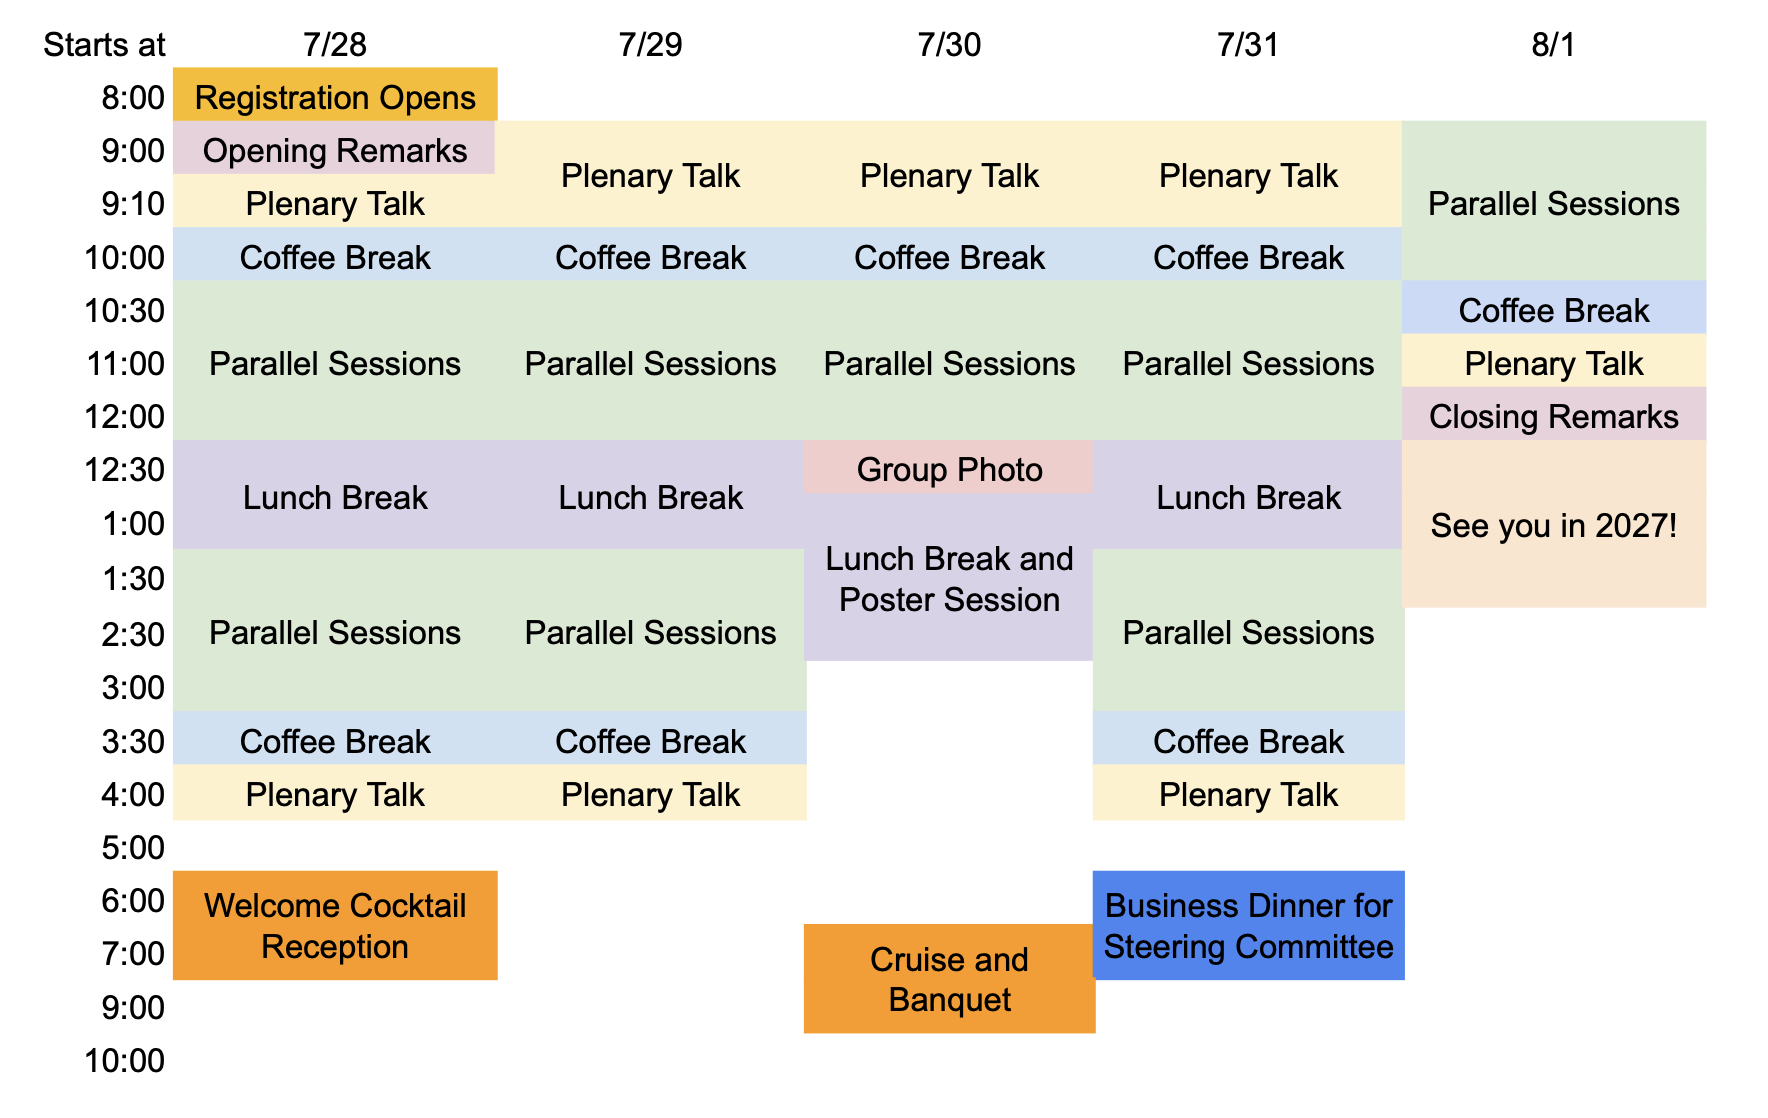
\includegraphics[width =.95\textwidth]{schedulev3_1.png}
%     \caption{Tentative Schedule}
% \end{figure}

\begin{figure}[h]
    \centering
    \centerline{\textbf{Tentative Schedule}}
    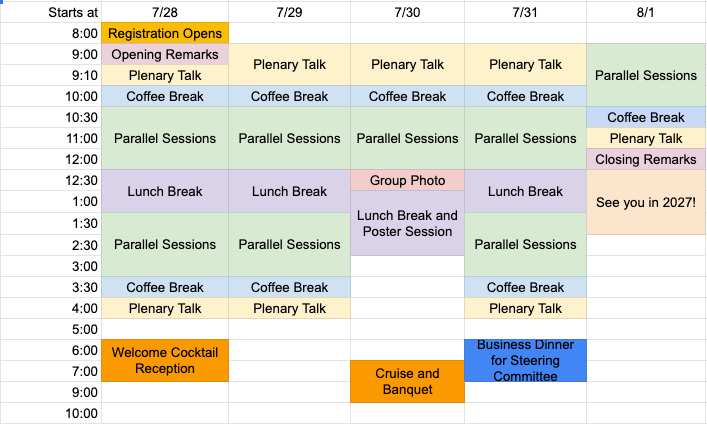
\includegraphics[width =.95\textwidth]{MCMSchedule.png}
\end{figure}

\section{Topics}
MCM 2025 will include active topics of research in Monte Carlo methods---those with a long history as well as those emerging topics.  These will include
\begin{itemize}
\item Markov chain Monte Carlo
\item Hamiltonian Monte Carlo
\item Sequential Monte Carlo, particle filters
\item Non-equilibrium candidate Monte Carlo
\item Bridge sampling
\item Rare event simulation
\item Multi-level Monte Carlo
\item (Randomized) quasi-Monte Carlo
\item Digital nets and lattice rules
\item Discrepancy theory
\item Complexity and tractability of multivariate problems
\item Variance reduction
\item Monte Carlo simulation on high-performance architectures
\item Uncertainty quantification
\item Experimental design
\item Generative models from artificial intelligence
\item Variational inference
\item Probabilistic numerics
\item Monte Carlo methods for quantum computers
\item Stochastic gradient and other stochastic optimization methods
\item Statistical learning and Monte Carlo sampling
\item Reinforcement learning and control
\item Bayesian inference
\item Computational statistical physics
\item Economic, engineering, industrial, and scientific applications
\end{itemize}

%\ny{My question is: It seems Hamiltonian Monte Carlo is a method of MCMC. Should we list it as a separate topic?}


\section{Budget}
The registration fee is anticipated to be USD600 per person, with a reduced fee of USD250 for students.  The registration fee will include lunch, coffee breaks, and the conference dinner. Travel and accommodation for plenary speakers will be covered up to USD2500 each.  We are planning for 150 participants paying the regular registration fee and 50 paying the student registration fee.

When it is confirmed that MCM 2025 will be held in Chicago, the local organizers will seek sponsorship from \href{https://www.imsi.institute}{Institute for Mathematical and Statistical Innovation}, an US National Science Foundation research institute based at the University of Chicago, and two research centers at IIT: the  \href{https://cos.iit.edu/cisc/}{Center for Interdisciplinary Scientific Computation} and the \href{https://mypages.iit.edu/~duan/LSD.html}{Center for Stochastic Dynamics}.

%Jeanette R. Massura, Director, Event Services, jmassura@iit.edu

%Ken Johnston, Interim Controller, 312.567.5850 johnston@iit.edu




\begin{figure}[h]
    \centering
    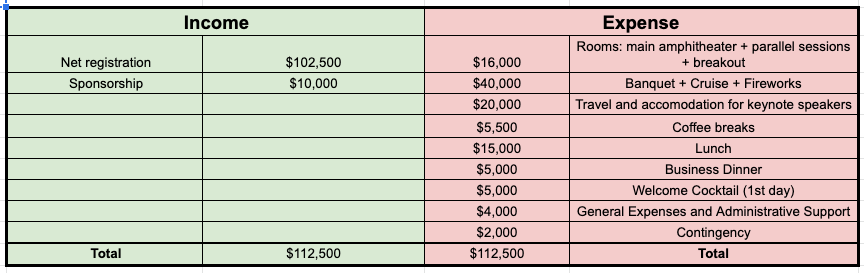
\includegraphics[width =.95\textwidth]{MCMBudget.png}
\end{figure}


\section{History of conferences}
\begin{itemize}
\item Paris, France, July 2023
\item  Mannheim, Germany, August 2021
\item Sydney, Australia, July 2019
\item Montreal, Canada, July 2017
\item  Linz, Austria, July 2015
\item  Annecy-le-Vieux, France, July 2013
\item  Borovets, Bulgaria, August 2011
\item  Brussels, Belgium, September 2009
\item  Reading, UK, June 2007
\item  Tallahassee, USA, May 2005
\item  Berlin, Germany, September 2003
\item  Salzburg, Austria, September 2001
\item  Varna, Bulgaria, June 1999
\item  Brussels, Belgium, April 1997
\end{itemize}


\end{document}
